
\section{Metodología}
El repositorio de imágenes satelitales Landsat es amplio y diverso.  Si bien se constituye como una gran herramienta para la comunidad científica, su uso requiere un tratamiento previo.  De igual manera, la construcción de un modelo preliminar de biomasa a partir de información secundaria exige la selección y validación de diferentes técnicas de regresión disponibles.  Esta sección resume una metodología de cinco etapas para la construcción del modelo de biomasa para el departamento de Nariño.  La figura~\ref{fig:metodology} ilustra la metodología propuesta. A continuación se explica en más detalle cada una de las etapas.

\begin{figure}
  \centering
  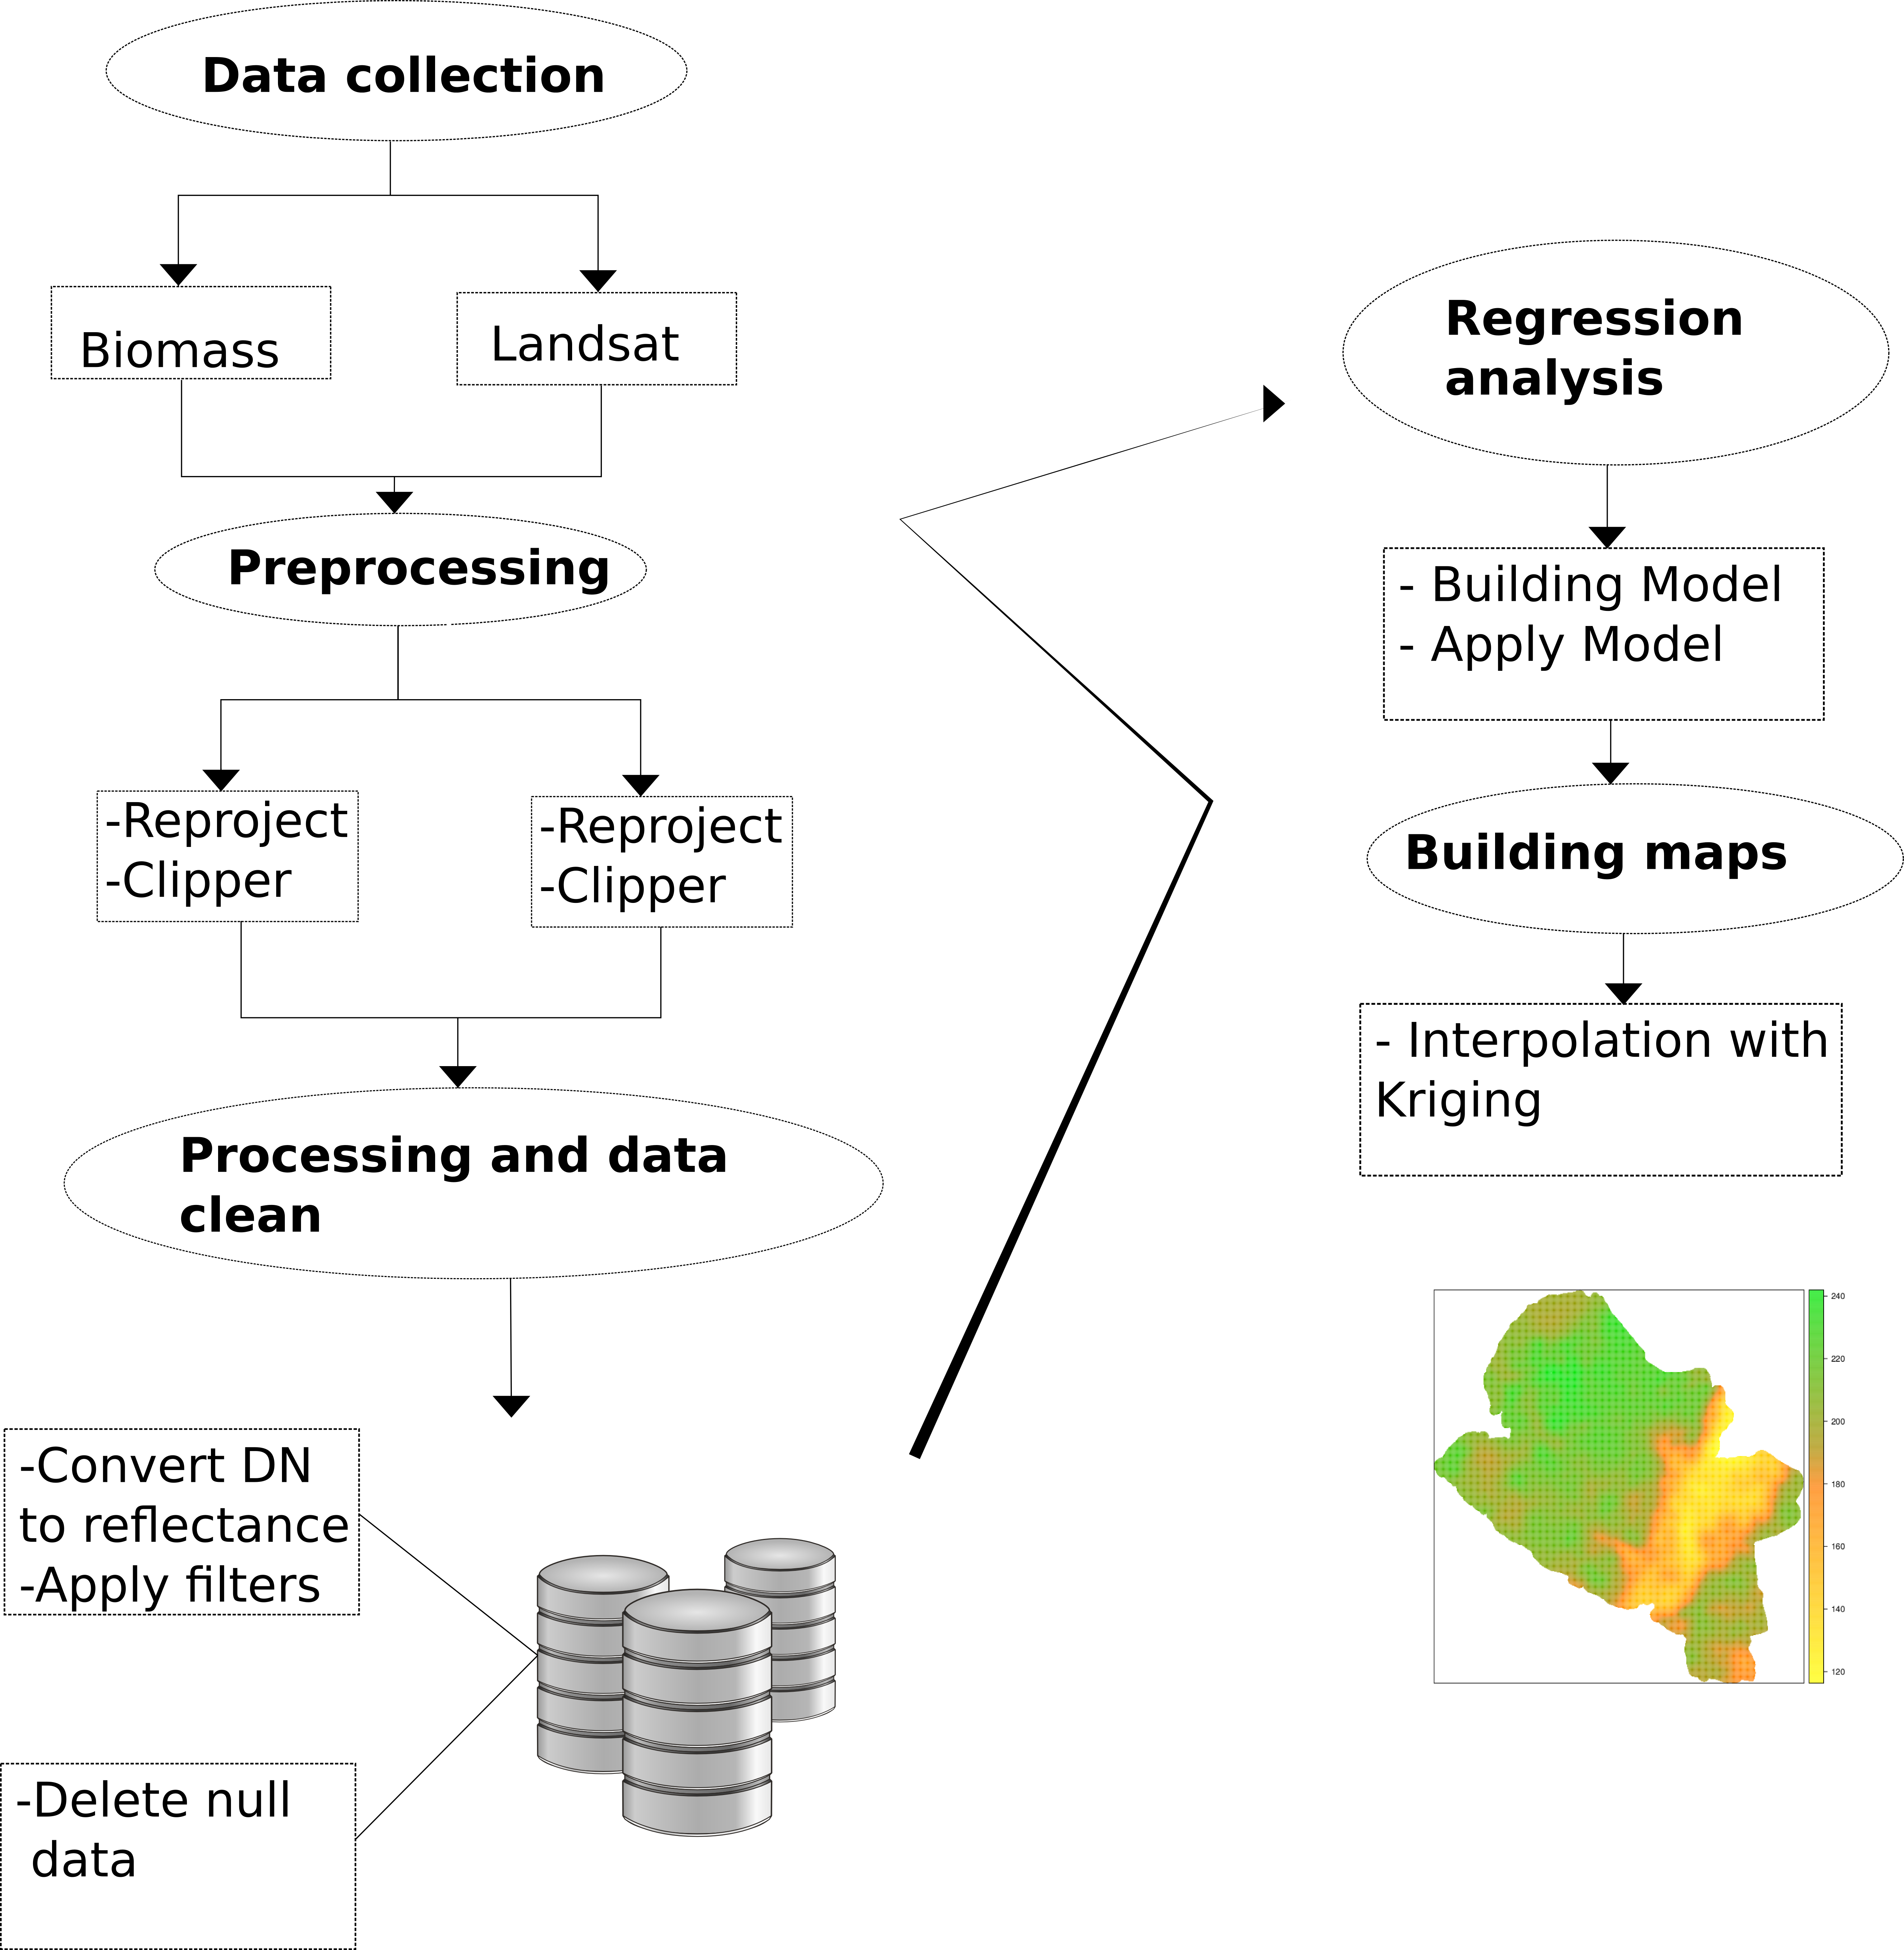
\includegraphics[width = 0.5\textwidth]{metodology.png}
  \caption{Metodología}
  \label{fig:metodology}
\end{figure}

\subsection{Obtención de datos}

El proceso de obtención de datos se realizó tomando imágenes satelitales proveidas por el sensor Landsat 7 ETM+. En este proceso se descargaron 1362 imágenes satelitales desde el año 1999 hasta mediados del año 2015. Para cubrir el departamento en su totalidad fue necesario descargar imágenes de cinco escenas diferentes.  La figura \ref{fig:cuts}a detalle los respectivos identificadores (Path ID y Row ID) y extensión de cada una de las escenas usadas.

Igualmente, durante esta etapa se tuvo acceso al mapa de biomasa construido por \cite{baccini2008afirst}.  Este es un mapa con resolución espacial de 1 $Km^2$ construido a partir de un modelo basado en imágenes MODIS recolectadas durante el año 2000 y 2003.

\subsection{Preprocesamiento}

En esta etapa se realizó un trabajo básico de procesamiento sobre las imágenes adquiridas.  Primero, dada la extensión del área de estudio, las escenas descargadas tenían diferentes sistemas de coordenadas (EPSG:32618 y EPSG:32617).  Por motivos de visualización se decidió unificar el sistema de coordenadas usando EPSG:3857, popular entre las herramientas de mapeo y desarrollo de aplicaciones web.  Muchas de las escenas cubrían una gran área del Océano Pacifico así como de otros departamentos de la región.  Se recorto las imágenes para contener solo los datos referentes al departamento de Nariño.  La figura \ref{fig:cuts}b ilustra el resultado final de esta etapa.

\begin{figure}
  \centering
  \subfigure[Imágenes Satélitales de Nariño]{\label{Imágenes Satélitales Nariño} 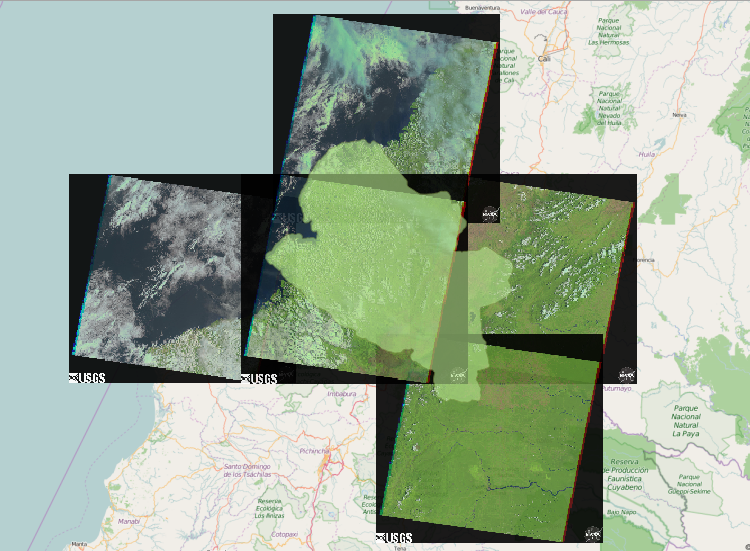
\includegraphics[width= 7cm]{cut1.png}}
  \vfill
  \subfigure[Imágenes recortadas de Nariño]{\label{Imágenes recortadas de Nariño}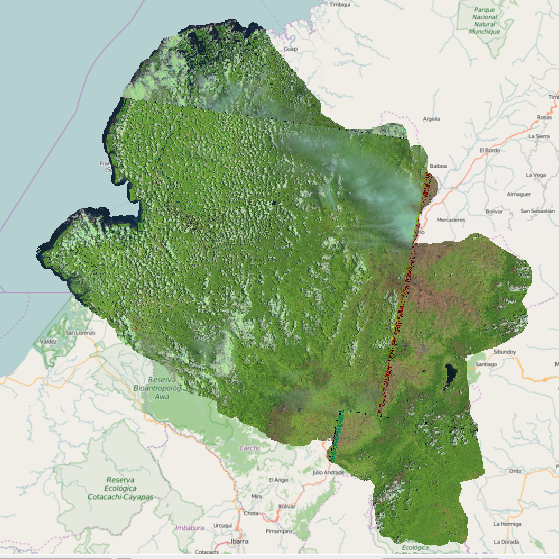
\includegraphics[width= 7cm]{cut2.png}}
  \caption{Prepocesamiento}
  \label{fig:cuts}
\end{figure}

De igual manera este proceso se lo realizó para el mapa de biomasa, como se muestra en la figura~\ref{fig:mapaNarino}

\begin{figure}
  \centering
  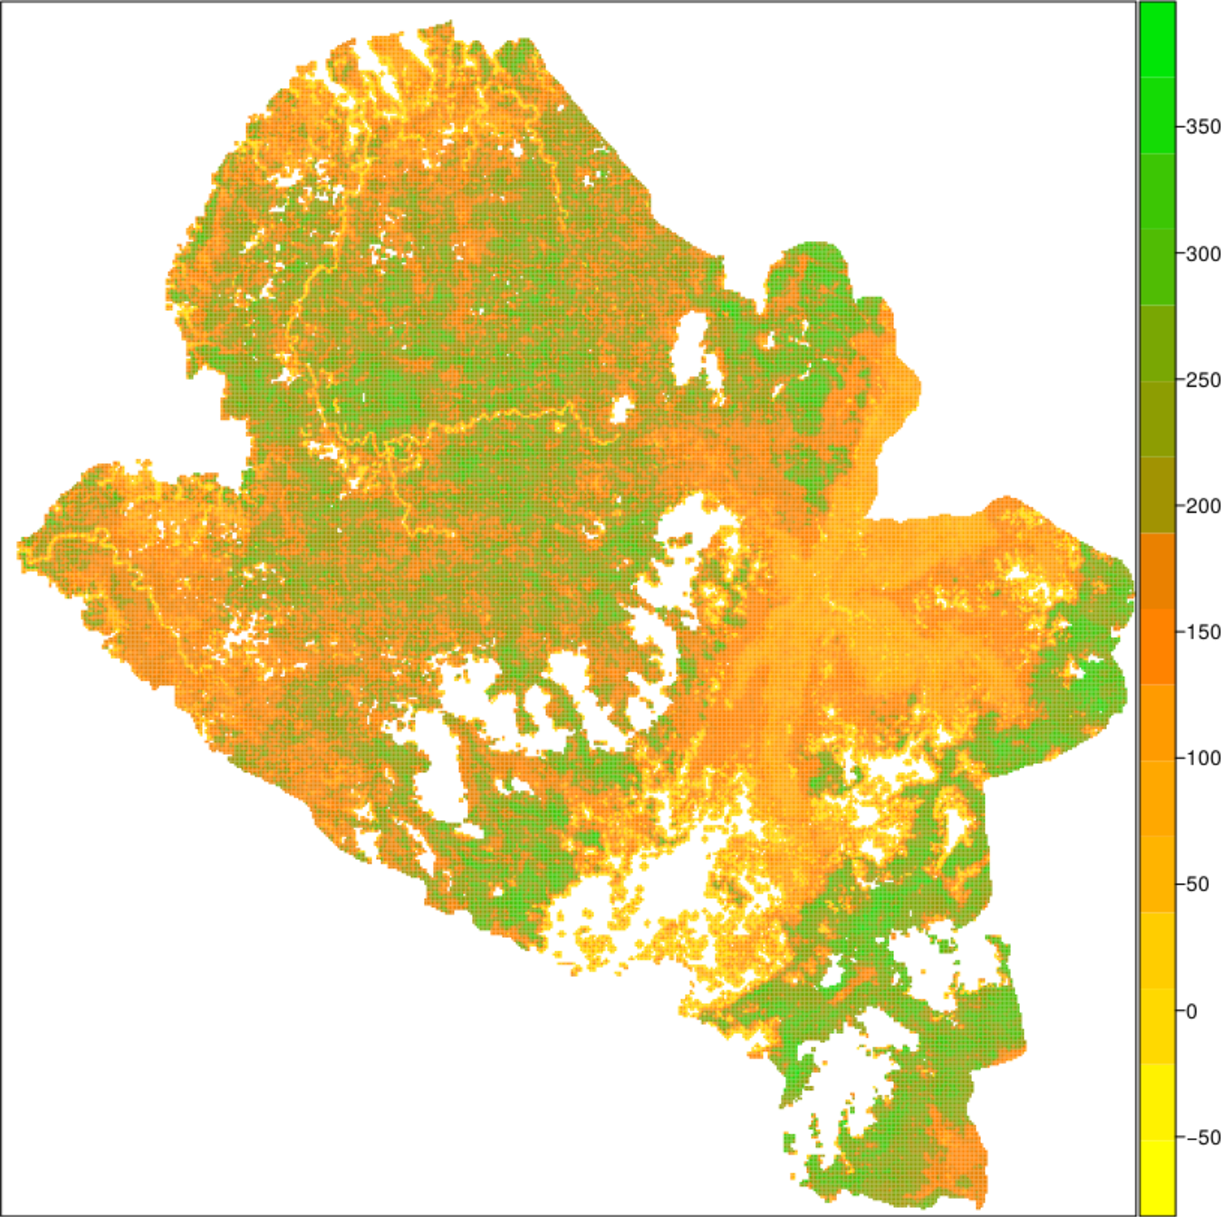
\includegraphics[width = 8cm]{mapaNarino.pdf}
  \caption{Mapa de biomasa en Nariño de 2000-2003 \cite{baccini2008afirst}}
  \label{fig:mapaNarino}
\end{figure}

\subsection{Procesamiento y limpieza de datos}

Con el objetivo de organizar los datos adquiridos se diseñó una base de datos a partir de cuatro entidades fundamentales: la fecha de la toma, los valores de reflectancia solar, los valores correspondientes de biomasa y las ubicaciones descartadas durante la limpieza de datos.  La figura \ref{fig:landsatET} ilustra el diseñó de la base de datos y los detalles de cada tabla se comentan a continuación:

\begin{figure}
  \centering
  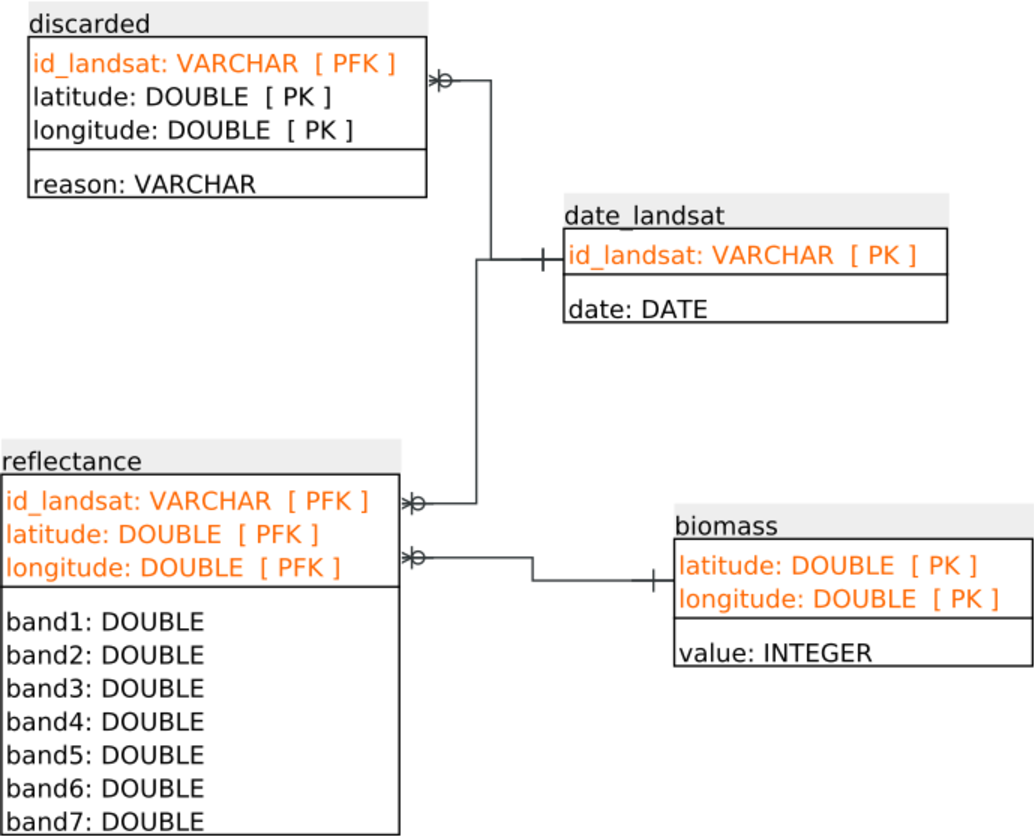
\includegraphics[width = 8cm]{landsatET.pdf}
  \caption{Modelo entidad-relacion Landsat}
  \label{fig:landsatET}
\end{figure}

\begin{itemize}
 \item Tabla date\_landsat: en la cual se almacenan las fechas de las imágenes satelitales.
 \item Tabla reflectance: en la cual se almacenan los datos capturados y convertidos a reflectancia solar, de las bandas Landsat (1-5 y 7) y la temperatura en grados kelvin de la banda 6.
 \item Tabla discarded: en la cual se almacenan los datos que fueron descartados por diversas razones (son puntos nublados, datos ambiguos o no corresponden a vegetación).
 \item Tabla biomass: en la cual se almacenan los datos de biomasa extraídos de \cite{baccini2008afirst}.
\end{itemize}

El procesamiento de las imágenes y alimentación de la base de datos se realizó a través de scripts y archivos procesados por lotes.  Entre los procesos realizados se transformó los valores originales extraídos de las imágenes (o digital numbers) a su correspondiente valor de reflectancia solar.  Se utilizó el algoritmo propuesto en \cite{irish2000landsat} para detectar puntos nublados en la zona clasificándolos como nubes frías, calientes o ambiguas.  Estos puntos se almacenaron con la intención de realizar posteriores estudios de nubosidad.  Finalmente, se aplicó un filtro adicional para calcular en índice NDVI (Normalized Difference Vegetation Index) con el objetivo de trabajar solo con aquellos puntos relacionados con vegetación y excluir áreas como cuerpos de agua o ciudades.  La tabla~\ref{tab:datos} muestra la relación de los datos obtenidos en este proceso.

\begin{table}
\caption{Datos obtenidos en en el proceso de procesamiento y limpieza  de datos}
\label{tab:datos}
\centering
%\scalebox{0.7}{
\begin{tabular}{c c c}
\toprule
 Nombre & Valor& Detalle  \\
\midrule
Datos biomasa & 81.993 & Registros biomasa \\
 & & (años 2000 a 2003 \cite{baccini2008afirst})\\
Datos biomasa usados & 140018 & construcción del modelo\\
\hline
Imágenes Landsat& 1321 & Imágenes de Nariño\\
procesadas & & (2000 a 2014) \\
Nube caliente & 3.731.768 & Registros 2000 a 2014 \\
Nube Fria & 27.827.009 & Registros 2000 a 2014 \\
No vegetación & 3.459.210 & Registros 2000 a 2014 \\
Ambiguo & 11.987.340 & Registros 2000 a 2014 \\
\hline
Total Datos Descartados & 47.005.327 & Total datos descartados \\
Datos Validos Reflectance & 4.071.185 & Registros 2000 a 2014 \\
\hline
Datos Totales & 51.076.512 & Registros Totales\\
& & (año 2000 a 2014) \\
\bottomrule
\end{tabular}
%}
\end{table}

\subsection{Análisis de regresión}

El análisis de regresión se realizó tomando los valores de las bandas Landsat obtenidas entre los años 2000 y 2003 y adicionando los valores correspondientes de biomasa para cada ubicación, dichos valores  se extrajeron de \cite{baccini2008afirst}.  Para poder obtener una mayor confiabilidad en el modelo solo se tuvo en cuenta aquellas ubicaciones con un número significativo de muestras.  Dada la alta nubosidad de la zona, muchos de los puntos contaban con pocas lecturas.  Por lo tanto, se consolidó un nuevo conjunto de datos con el promedio de aquellos puntos que superaban al menos un número considerable de lecturas validas.  

Se construyeron diferentes modelos, iterando el número de muestras por cada punto entre 10 y 45.  El mejor modelo se obtuvo cuando el número de muestras superaba las 35 lecturas.  El conjunto de datos final arrojó 1009 registros válidos.  El comportamiento en las demás iteraciones indica que con pocas muestras el conjunto de entrada es altamente hetereogeneo, guiado por aquellos puntos con pocas lecturas y alta variabilidad.  En cambio, al aumentar el número de lecturas, la variabilidad de las muestras baja pero con el alto riesgo de sobrecargar el modelo (\cite{babyak_what_2004}). 

Antes de aplicar las técnicas de regresión, se procedió a evaluar la calidad y relevancia de las bandas de las imágenes Landsat con el objetivo de predecir valores de biomasa.  Se utilizó el algoritmo propuesto en \cite{kursa2010feature} para la extracción y evaluación de atributos. El algoritmo está diseñado como un recubrimiento alrededor del algoritmo de clasificación \texttt{random forest} y califica cada atributo en el conjunto de datos de acuerdo a su importancia a la hora de clasificar el atributo buscado. En la figura~\ref{fig:boruta} se puede observar la relevancia de todas las bandas Landsat (en verde) que se ubican por encima de los valores por defecto (en azul).  Esto indica que la relevancia de las bandas de las imágenes Landsat esta por encima del azar. Concluimos que todas las bandas resultan importantes a la hora de modelar biomasa.

\begin{figure}
  \centering
  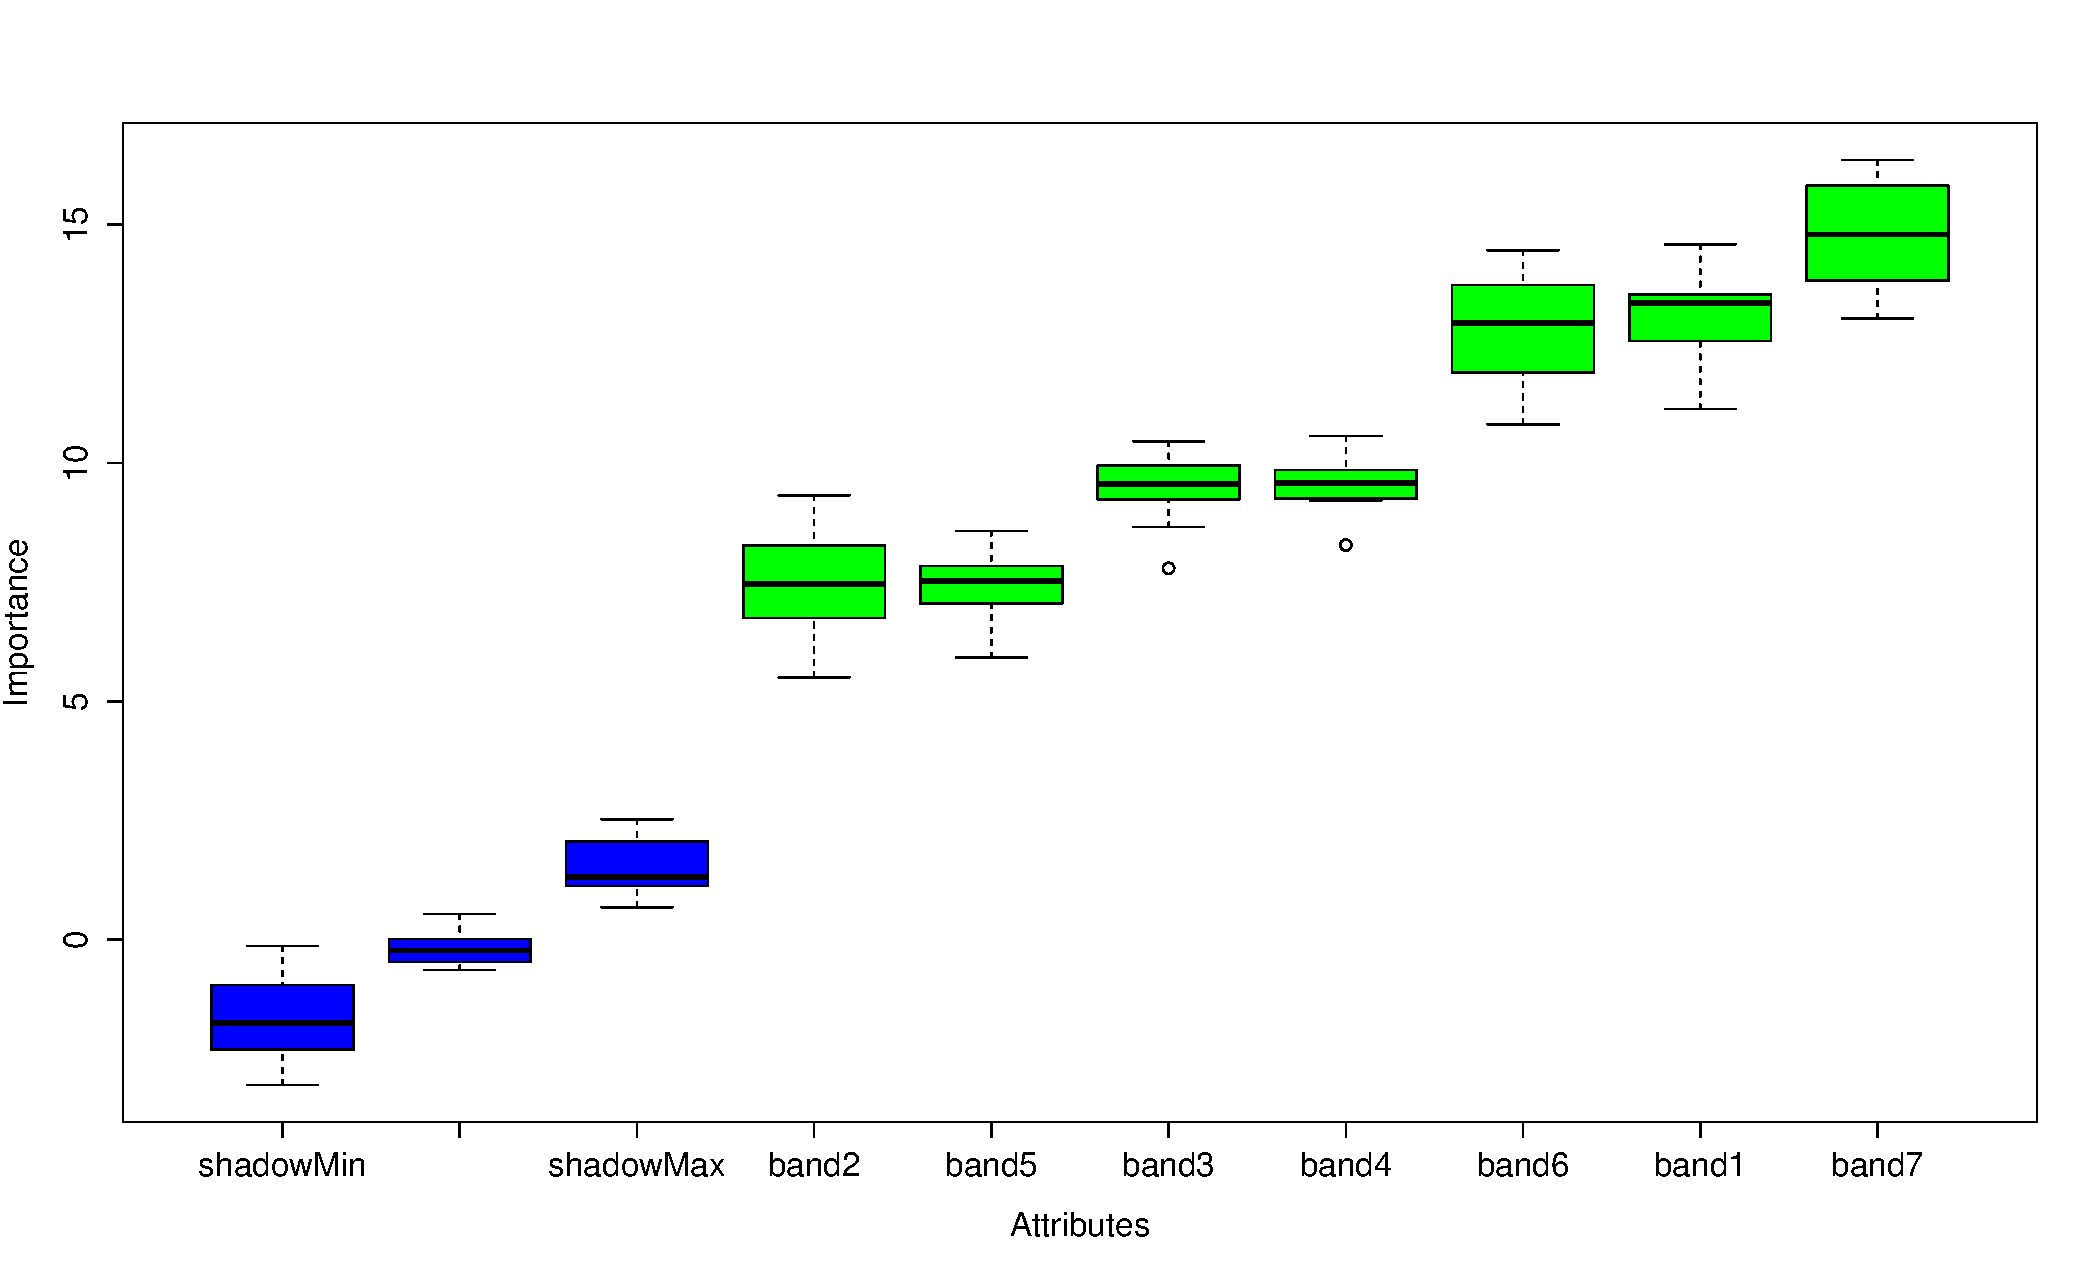
\includegraphics[width = 8cm]{boruta.pdf}
  \caption{Relevancia de bandas Landsat en el análisis de regresión}
  \label{fig:boruta}
\end{figure}

Con un nuevo conjunto de datos definido y evaluado, se continuó con la construcción de modelos de regresión utilizando diversas técnicas de análisis.  La biblioteca de código abierto \texttt{rminer}, presentada por \cite{cortez2010data} para la herramienta R, provee diferentes implementaciones y una interfaz que facilita la ejecución de diferentes pruebas y la extracción de modelos y sus correspondientes métricas de evaluación.  

Se construyó un total de 13 modelos y se evaluaron 6 metricas por cada uno. La tabla \ref{tab:metricas} ilustra los resultados obtenidos. Las técnicas utilizadas fueron: ctree (conditional inference tree), rpart (decision tree), kknn (k-nearest neighbor), mlp (multilayer perceptron with one hidden layer), mlpe (multilayer perceptron ensemble), ksvm (support vector machine), randomForest (random forest algorithm), mr (multiple regression), mars (multivariate adaptive regression splines), cubist (rule-based model), pcr (principal component regression ), plsr (partial least squares regression) y cppls (canonical powered partial least squares).  Las metricas evaluadas fueron: SAE (sum absolute error), MAE (mean absolute error), RAE (relative absolute error), RMSE (root mean squared error), COR (correlation) y R2 (coefficient of determination $R^2$).

\begin{table}
\caption{Métricas de modelos analizados. Los valores en negrilla indican los mejores resultados para cada métrica.}
\label{tab:metricas}
\centering
\scalebox{0.7}{
\begin{tabular}{c c c c c c c}
\toprule
 & SAE& MAE & RAE & RMSE & COR & R2 \\
\midrule
ctree & 10406.58225 & 30.88007 & 65.04650 & 40.02893 & 0.69401 & 0.48165 \\
rpart & 10197.95826 & 30.26100 & 63.74249 & 39.37592 & 0.70520 & 0.49730 \\
kknn & 9147.51425 & 27.14396 & 57.17667 & 36.86581 & 0.74955 & 0.56182 \\
mlp & 9179.79310 & 27.23974 & 57.37843 & 34.70711 & 0.78122 & 0.61031 \\
mlpe & 8746.27740 & 25.95335 & 54.66874 & 34.57953 & 0.78309 & 0.61323 \\
ksvm & \textbf{8462.61487} & \textbf{25.11162} & \textbf{52.89570} & 34.67742 & \textbf{0.79830} & \textbf{0.63729} \\
randomForest & 8807.76477 & 26.13580 & 55.05306 & 34.70615 & 0.78239 & 0.61214 \\
mr & 10410.13919 & 30.89062 & 65.06873 & 38.61068 & 0.72000 & 0.51840 \\
mars & 8842.91866 & 26.24011 & 55.27279 & \textbf{33.96852} & 0.79161 & 0.62665 \\
cubist & 9012.54150 & 26.74345 & 56.33302 & 35.70576 & 0.77611 & 0.60235 \\
pcr & 10337.63121 & 30.67546 & 64.61552 & 38.59290 & 0.72023 & 0.51873 \\
plsr & 10337.63121 & 30.67546 & 64.61552 & 38.59290 & 0.72023 & 0.51873 \\
cppls & 10337.63121 & 30.67546 & 64.61552 & 38.59290 & 0.72023 & 0.51873 \\
\bottomrule
\end{tabular}}
\end{table}

\subsection{Construcción de mapas}

A partir de los resultados de la tabla \ref{tab:metricas} durante la construcción de mapas se utilizó el modelo \texttt{ksvm}.  Para la construcción de mapas de biomasa se utilizó el método Kriging (\cite{bivand_applied_2013, cressie_statistics_2015}).  Kriging provee una solución al problema de la estimación basada en un modelo continuo de variación espacial estocástica.  El objetivo de Kriging es el de estimar el valor de una variable aleatoria, en este caso biomasa, en uno o más puntos no muestreados o sobre grandes bloques. 

El método Kriging recibe como entrada datos de la muestra y una malla dependiendo de la resolución que se quiera obtener. Para ello, se obtuvo una muestra de los datos obtenidos al aplicar el modelo seleccionado a datos agregados por mes y año y un mapa general que abarca el periodo de estudio.  La malla se construyó con puntos regulares espaciados cada 450 metros. En la figura~\ref{fig:biomasaMes}, figura~\ref{fig:biomasaAnio}, figura~\ref{fig:biomasaTotal}  se muestra los mapas obtenidos por meses, años y general respectivamente. 
 
\begin{figure}
  \centering
  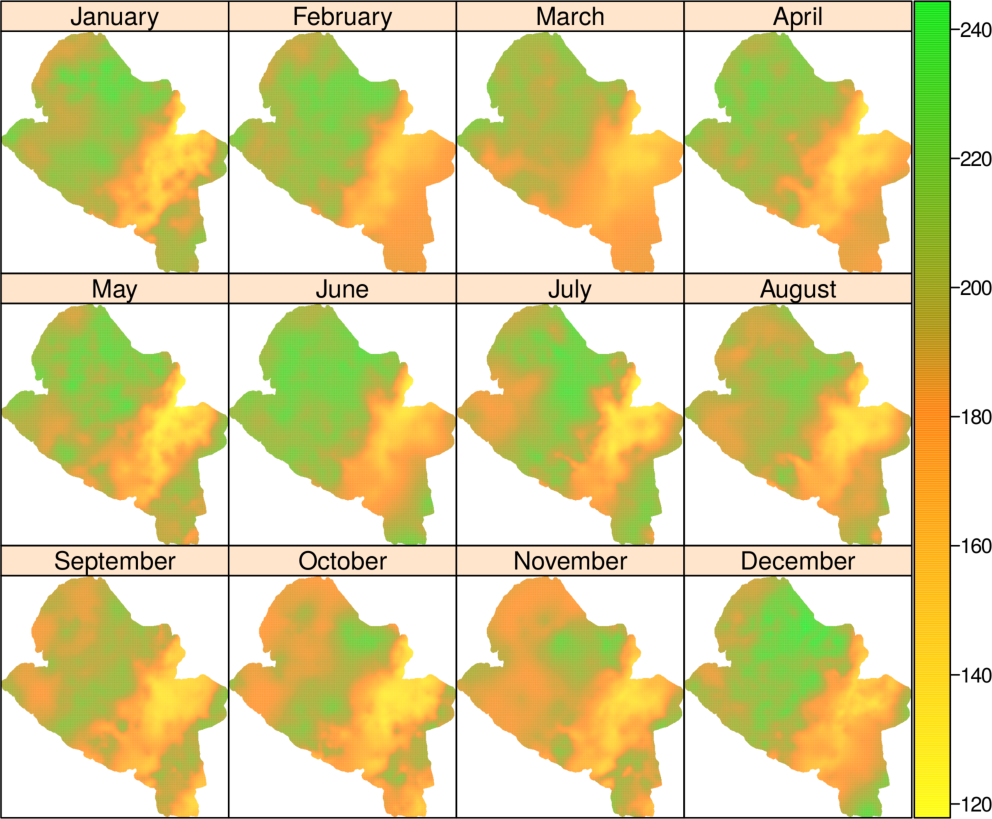
\includegraphics[width = 8cm]{mapMonthsBiomass.pdf}
  \caption{Mapas biomasa por meses}
  \label{fig:biomasaMes}
\end{figure}

\begin{figure}
  \centering
  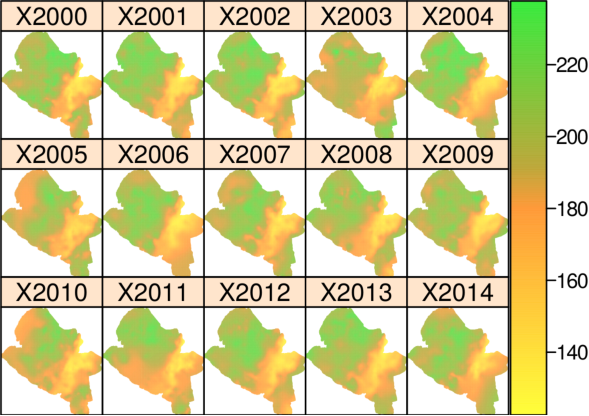
\includegraphics[width = 8cm]{mapYearsBiomass.pdf}
  \caption{Mapas biomasa por años}
  \label{fig:biomasaAnio}
\end{figure}

\begin{figure}
  \centering
  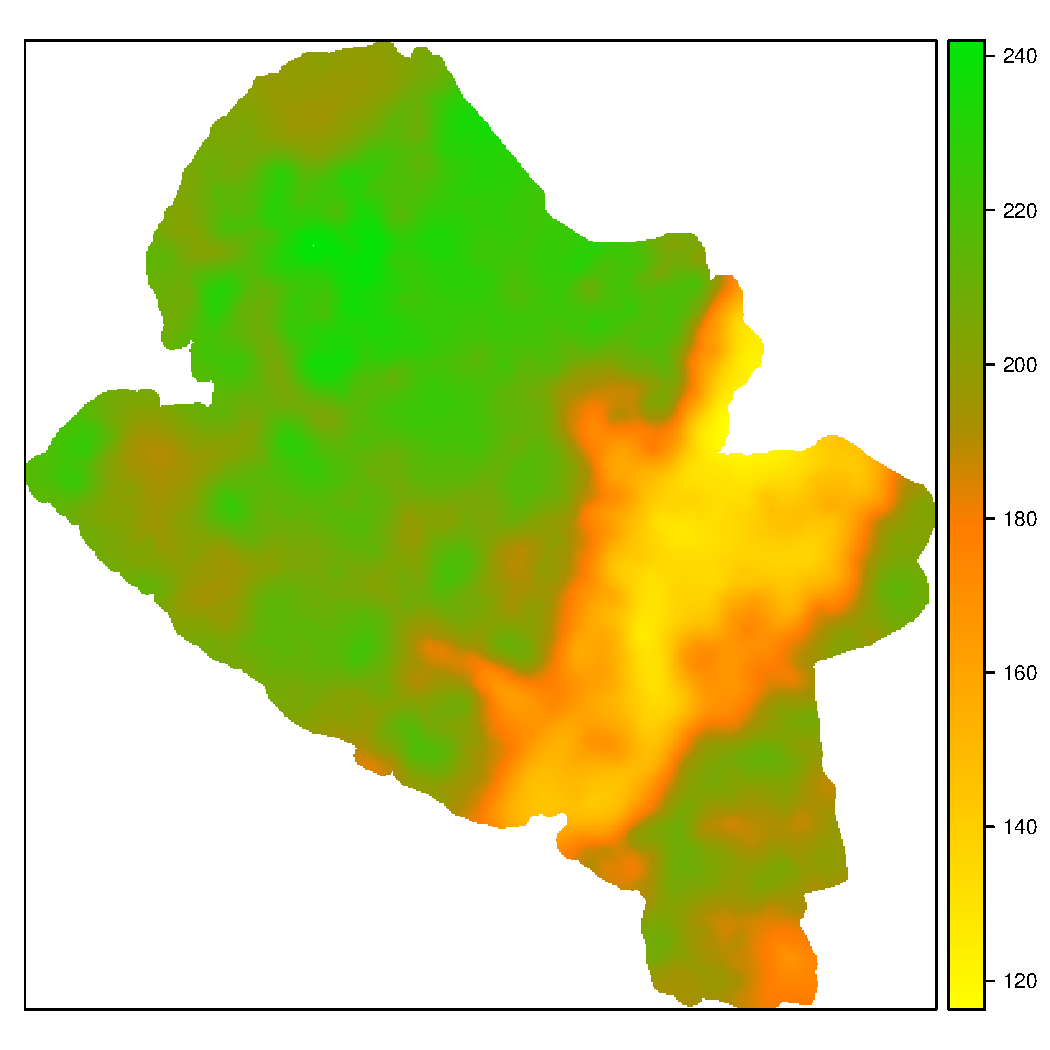
\includegraphics[width = 8cm]{mapGeneralBiomass.pdf}
  \caption{Mapas biomasa general años 2000-2014}
  \label{fig:biomasaTotal}
\end{figure}
